

\section{Organisation du projet}


% Travail en équipe
\subsection{Organisation du travail en équipe}

% Problématique
\subsubsection*{Problématique}

    Le travail en équipe n'est pas une chose évidente, et il est nécessaire de mettre en
place une méthode afin d'optimiser notre productivité, sinon cas nous le risque de 
malencontreusement traiter d'un même sujet séparément, et se rendre compte qu'on a perdu notre
temps.

% Solutions
\subsubsection*{Solutions mises en place}

\subsubsection*{Méthode Kanban}

    Nous avons utilisé l'application web kanboard, installée sur un serveur personnel, afin de
distribuer le travail à faire, ainsi nous savions à tout moment, ce qu'il y avait à faire,
ce qui était en train d'être fait et ce qui avait été fait. 


\subsubsection*{Utilisation de git}

    L'utilisation d'un gestionnaire de version est essentiel pour la 
réalisation de ce genre de projet. Cependant, se limiter à une utilisation élémentaire
de ce logiciel pour le travail en équipe peut mener à une multiplication de problèmes de 
conflits, pouvant entraver l'avancée du projet. 

    Plusieurs solutions plus ou moins élaborées pouvaient être mises en place, nous avons opté 
pour un entre-deux: nous utilisions 3 branches : la branche master, qui se devait d'être 
propre, le code qui s'y trouvait devait toujours être
compilable, et devait contenir le moins de bugs possible. Les deux autre branches que nous
utilisions nous étaient attitrées, à chaque fois que nous nous attribuions une tache sur le
kanboard, nous développions une solution sur notre branche puis nous fusionnions sur la branche
master.

Schématiquement, notre utilisation de git se résume au schéma suivant :

\begin{center}
    \begin{figure}[H]
        \centering
        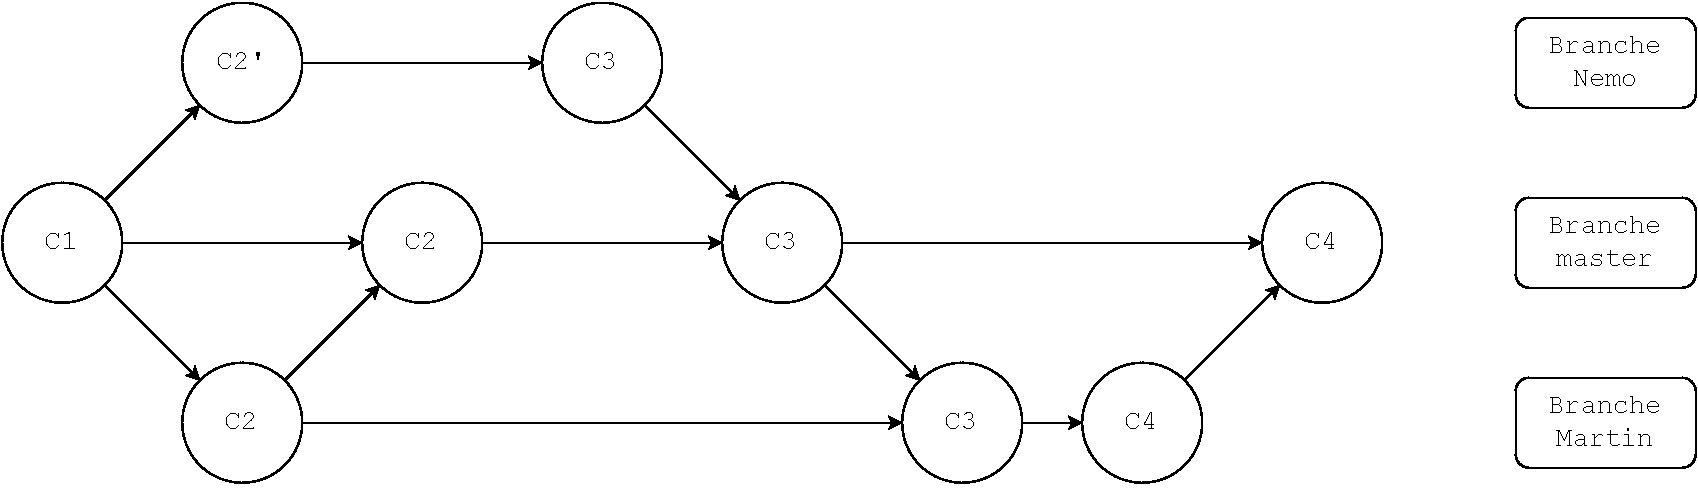
\includegraphics[width=\textwidth]{img/git_branch.pdf}
        \caption{Utilisation de nos 3 branches de git}
        \label{fig:git_branch}
    \end{figure}
\end{center}


% Organisation Code
\subsection{Organisation du code}


\subsubsection*{Problématique}


    Un projet d'une telle envergure nécessite une organisation spéciale afin d'être mené à 
bien. Il s'agit d'une organisation qui doit faciliter l'ajout de nouvelle fonctionnalités,
faciliter la modification de fonctionnalités déjà présente et faciliter la lecture et la 
compréhension de ce qui a déjà été fait.




\subsubsection*{Solutions mises en place}


\subsubsection*{Division en dossiers principaux}


    Sachant que nous nous apprêtions à créer un exécutable pour le projet en lui-même et pour les
tests, nous avons décidé de séparer les sources pour chaque exécutable dans un dossier séparé.


    Ainsi, notre projet est constitué de 4 dossiers principaux: \code{/src}, \code{/tst}, 
\code{/cli\_src}, \code{/evaluator\_src}, comme le schématise le schéma ci-dessous


\begin{center}
    \begin{figure}[H]
        \centering
        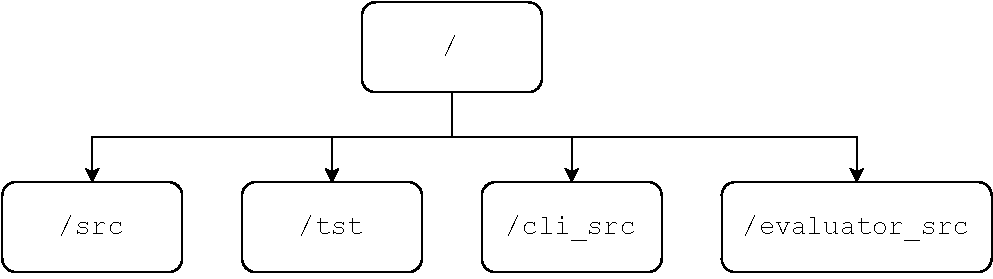
\includegraphics[width=.5\textwidth]{img/main_directories.pdf}
        \caption{Schéma des dossiers principaux du projet}
        \label{fig:main_dirs}
    \end{figure}
\end{center}




\subsubsection*{Division du code par thème}


    Une fois qu'on a divisé en dossiers principaux, on divise le code
dans des sous-dossiers au sein de ces dossiers. Ainsi, on va avoir un
sous-dossier pour les builders et la structure de guilde, un pour les 
tokens et la structure de markets etc... On a aussi un sous-dossier \code{/src/utils},
qui va contenir toutes les structures et fonctions génériques, comme
une structure de file ou une macro \code{MIN} qui retourne le minimum entre 2 entiers.

    L'architecture des sous-dossiers de \code{/src} est schématisé ci-dessous :


\begin{center}
    \begin{figure}[H]
        \centering
        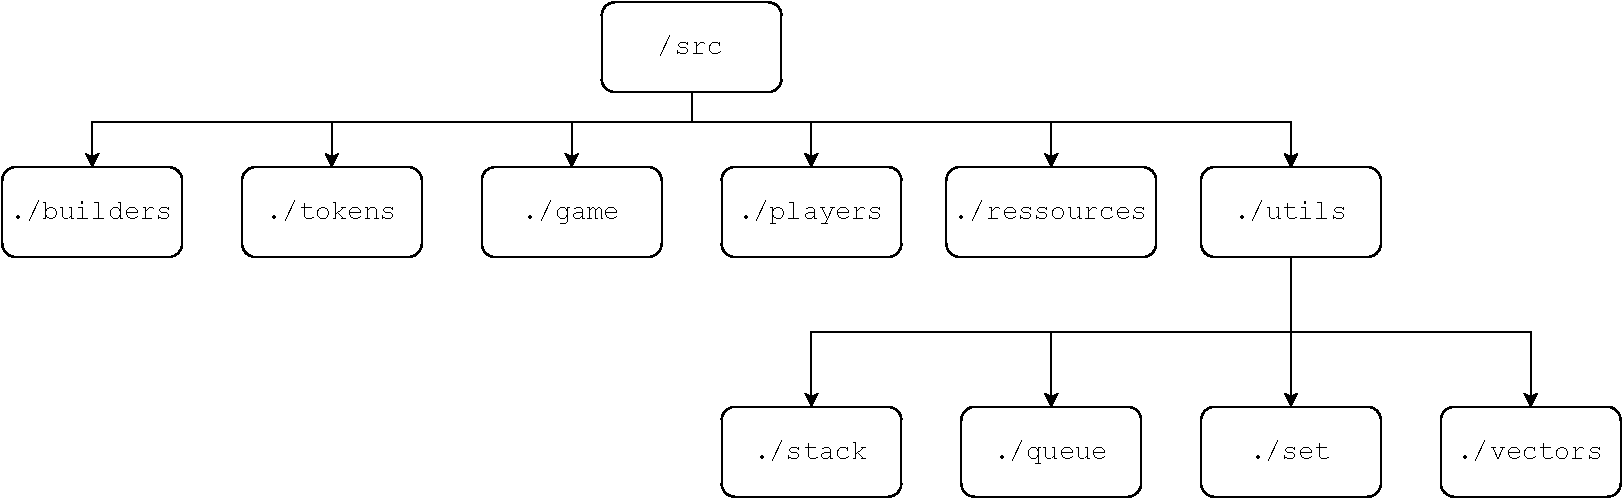
\includegraphics[width=.8\textwidth]{img/src_sub_dir.pdf}
        \caption{Schéma sous-dossiers de $/src$}
        \label{fig:src_sub_dirs}
    \end{figure}
\end{center}




\subsubsection*{Mise en place d'une convention}


\subsubsection*{Problématique}


    Le travail en groupe fait qu'on se retrouve tôt ou tard à lire ou à utiliser des outils codés par une 
autre personne. Ainsi, la forme du code requiert une certaine attention afin de rendre l'utilisation de ces
outils naturelle et la lecture du code uniforme.


\subsubsection*{Solution mis en place}

    Pour résoudre ce problème de forme, on a mit en place une convention de nommage pour les
variables et les fonctions, ainsi que des règles d'écriture. 

    Nous avons décidé d'utiliser la convention \code{snake\_case} pour ce qui est de la forme,
nous nommons les types \lstinline{struct type_t} afin de ne pas les confondre avec d'éventuelles variables.
Une fonction qui devait s'appliquer à un type \lstinline{struct type_t} en particulier est notée
\lstinline{type_function(...)}.

    Vous trouverez ci-dessous des exemples non-exhaustif de la mise en pratique de ces conventions

\begin{lstlisting}[frame=single, caption={Exemples de mise en pratique de ces conventions}]
struct queue_t ;


unsigned int queue_append(struct queue_t* queue, void* value);
\end{lstlisting}




\subsubsection*{Compilation}


\subsubsection*{Problématique}


    Travailler avec telle structure de fichier rend la compilation moins évidente, et fastidieuse si on voulait 
la faire manuellement avec \code{gcc}.


\subsubsection*{Solution mis en place}

    Nous avons utilisé \code{make}, et nous nous sommes appliqué à l'écriture d'un \code{makefile} qui
permettrait d'avancer sereinement dans le projet.

    Notons avant tout que notre \code{makefile} est largement inspiré des ébauches proposées du \href{https://spin.atomicobject.com/makefile-c-projects/}{poste de blog de Job Vranish}, 
ces ébauches formait une fondation solide sur laquelle travailler. Cependant, nous nous sommes tout de même donné le mal de nous l'approprier
afin de l'adapter à notre structure peut-être originale.

    Comme la plupart des sources du dossier \code{/src} sont partagées entre chaque exécutables, nous avons fait le choix de
d'abord chercher tous les fichiers sources de \code{/src}, puis de retirer le fichier \code{/src/projet.c} contenant la fonction main.

\begin{lstlisting}[frame=single, language=sh, caption={Filtrage des fichiers sources du jeu}]
SRC_DIRS := ./src
PROJECT_MAIN_FILE_NAME := ./src/project.c

SRCS := $(shell find $(SRC_DIRS) -name '*.c')
SRCS := $(filter-out $(PROJECT_MAIN_FILE_NAME), $(SRCS))
\end{lstlisting}

    Nous avons opté pour l'utilisation de l'option \code{-Isous\_dossier} de \code{gcc}, permettant de déclarer des librairies systèmes. Ainsi, en 
l'utilisant avec tous les sous-dossiers de \code{/src} et des autres dossiers principaux, cela nous permet de nous limiter à l'écriture de `\lstinline[language=C]{#include "fichier.h"}` dans nos fichiers sources plutôt que le chemin relatif vers le fichier \code{fichier.h}. Étant donné notre arborescence complexe, cela simplifie largement la lecture et l'écriture des dépendances.

    Cependant, il fallait aussi que nos éditeurs, par le biais de clang, puissent être utilisable. D'où l'ajout de la target \code{clang\_custom\_lib\_support} dans
le makefile, permettant de créer le fichier de configuration \code{compile\_flags.txt} indiquant nos librairies systèmes personnalisées à clang.

Finalement l'utilisation d'un nouveau dossier, le dossier \code{/build}. Ce dernier nous sert à stocker tous les fichiers de compilation. Afin de les stocker, nous recréons la structure précédente du fichier, comme le schématise la figure \ref{fig:build_dir}. 

    L'utilisation de ce dossier permet d'avoir une séparation claire entre le reste du projet et la partie compilation.

\begin{center}
    \begin{figure}[H]
        \centering
        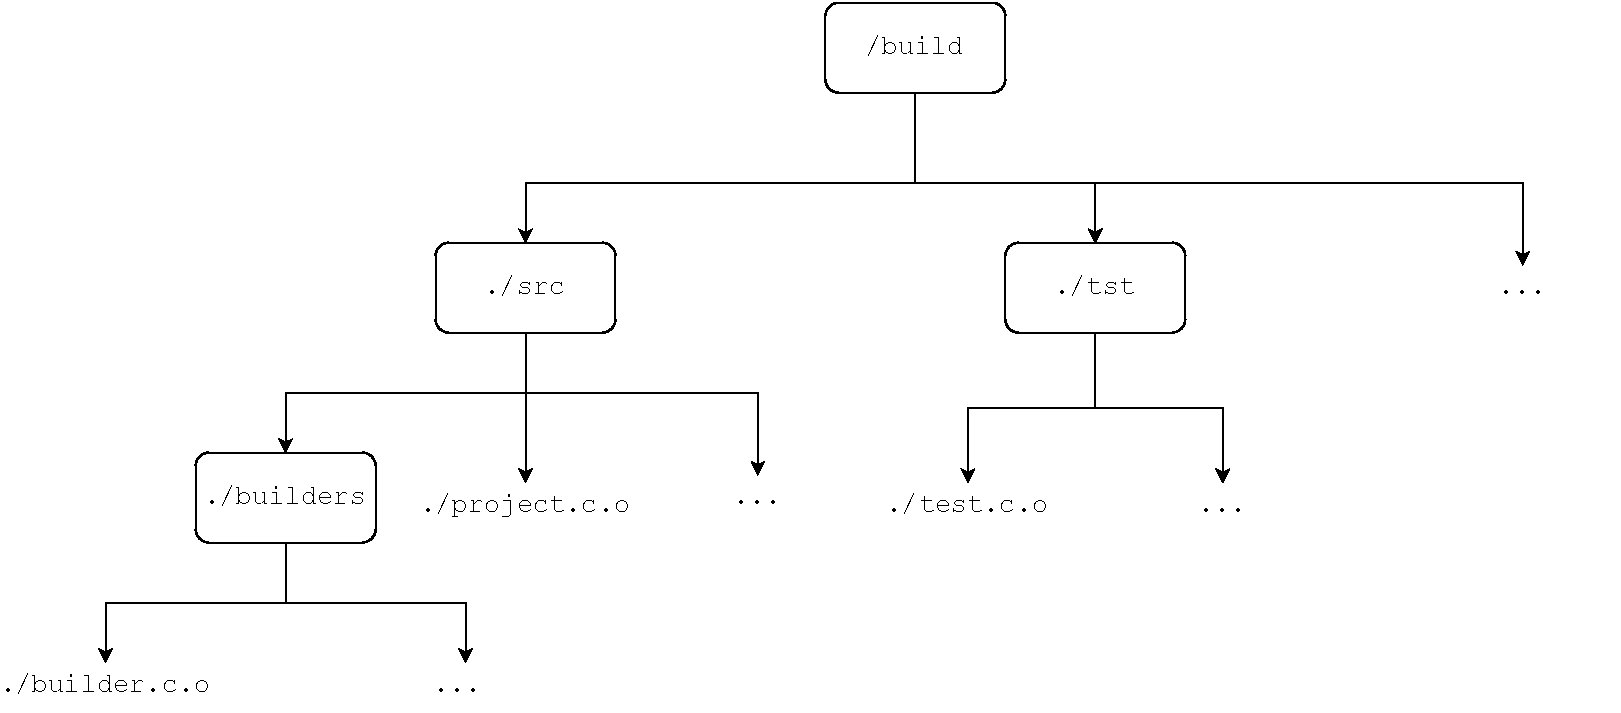
\includegraphics[width=.8\textwidth]{img/build_dir.pdf}
        \caption{Schéma arboressence du dossier /build}
        \label{fig:build_dir}
    \end{figure}
\end{center}


